% Keep the IEEE template's classic Times font encoding with either engine.
\RequirePackage[OT1]{fontenc}
\documentclass[conference,letterpaper]{IEEEtran}
\usepackage{cite}
\usepackage{amsmath,amssymb}
\usepackage{graphicx}
\usepackage{array}
\usepackage{textcomp}
\usepackage{url}
\newcolumntype{L}[1]{>{\raggedright\arraybackslash}p{#1}}
\makeatletter
\newcommand{\linebreakand}{%
  \end{@IEEEauthorhalign}\hfill\mbox{}\par
  \mbox{}\hfill\begin{@IEEEauthorhalign}}
\makeatother

\title{Boundary Supervision for Camouflaged Object and Industrial Defect Segmentation}
\author{
\IEEEauthorblockN{Shreyash Chilweri}
\IEEEauthorblockA{\textit{Department of CSE}\\
\textit{D. Y. Patil International University}\\Pune, India}
\and
\IEEEauthorblockN{Ganesh Sutar}
\IEEEauthorblockA{\textit{Department of CSE}\\
\textit{D. Y. Patil International University}\\Pune, India}
\linebreakand
\IEEEauthorblockN{Shreeyash Raut}
\IEEEauthorblockA{\textit{Department of CSE}\\
\textit{D. Y. Patil International University}\\Pune, India}
\and
\IEEEauthorblockN{Ketan Raut}
\IEEEauthorblockA{\textit{Department of CSE}\\
\textit{D. Y. Patil International University}\\Pune, India}
}
\begin{document}
\maketitle

\begin{abstract}
We compare the Frequency Injection Network with and without boundary supervision for camouflaged object segmentation and evaluate an independently trained industrial defect baseline. The added objective combines binary cross entropy and Dice loss on differentiable morphological boundaries. Both camouflage variants share their full initialization, data split and optimization settings and complete 200 epochs. The inference architecture remains unchanged at 3,742,988 parameters. On 404 validation images, final mean absolute error decreases from 0.044454 to 0.044046, while the common validation structure loss increases slightly. One held out camouflage image gives baseline and boundary Dice scores of 0.9621 and 0.9671. The industrial baseline gives Dice scores of 0.8702 and 0.9276 on two defective images and an empty mask on one normal image. The protocol defines preprocessing, losses, sampling and native resolution metrics; exported probability maps and masks include foreground error counts. The validation difference is small, and aggregate test performance and contour improvement remain unverified.
\end{abstract}
\begin{IEEEkeywords}
camouflaged object segmentation, frequency injection, boundary supervision, industrial defect segmentation
\end{IEEEkeywords}

\section{Introduction and Objectives}
Camouflaged object segmentation estimates which pixels belong to an object that resembles its background. Region overlap alone can hide contour errors: a mask may cover most of an object while placing its edge incorrectly. Frequency Injection Network (FINet) combines spatial and frequency features in a compact model~\cite{finet}. We retain that model and study an additional training objective that directly supervises local boundaries.

We isolate the effect of boundary supervision by matching the complete initial state and training budget while retaining the inference layers and parameter count. Native resolution probabilities and explicit region and contour metrics distinguish overlap from edge alignment. A separately trained industrial baseline tests the method under a declared supervised protocol. Numerical results and saved outputs allow each prediction to be checked against its original mask.

The A/B controls apply within each domain; data handling differs between domains (Table~\ref{tab:comparison}).

Both camouflage models completed 200 epochs and have validation histories and a same-image test demonstration. The industrial baseline also completed 200 epochs. An independently saved industrial boundary state is available for recovery, but a matched final industrial comparison is still unavailable. Completed training, validation measurements and individual test examples provide different levels of evidence.

\section{Background and Method}
\subsection{Prior Work and Problem Definition}
Liang \textit{et al.} introduced FINet to inject high and low frequency information into spatial features~\cite{finet}. Its encoder uses EfficientNet, a convolutional network family based on coordinated model scaling~\cite{efficientnet}. Our camouflage development data combine training images from COD10K~\cite{cod10k} and CAMO~\cite{camo}. The industrial extension uses MVTec AD~\cite{mvtec}, which was introduced for anomaly detection with normal training images. Using its defect annotations during training creates a different, supervised experiment.

Let an input photograph have native height $H$ and width $W$. FINet receives a resized image of $384\times384$ pixels and produces four logits maps $Z_h$, $h=1,\ldots,4$. The resized training mask is $G\in[0,1]^{384\times384}$. The structure loss receives $G$ unchanged, retaining soft camouflage targets. The boundary branch binarizes its target; industrial masks already have binary values. Individual example metrics use native binary annotations.

\subsection{Spatial and Frequency Inputs}
The RGB and frequency branches start from the same resized photograph but use different intensity scales. With RGB intensities $X_c\in[0,255]$, the spatial input is
\begin{equation}
 X^{\mathrm{rgb}}_c=\frac{X_c/255-\mu_c}{s_c},
 \label{eq:rgb}
\end{equation}
where the ImageNet normalization constants are
\[
 \mu=(0.485,0.456,0.406),\quad s=(0.229,0.224,0.225).
\]

The frequency branch retains the $0$ to $255$ scale and the exact color transform in the source implementation:
\begin{equation}
\begin{bmatrix}Y\\C_b\\C_r\end{bmatrix}
=
\begin{bmatrix}
0.257&0.564&0.098\\
-0.148&-0.291&0.439\\
0.439&-0.368&-0.071
\end{bmatrix}
\begin{bmatrix}X_R\\X_G\\X_B\end{bmatrix}
+
\begin{bmatrix}16\\128\\128\end{bmatrix}.
\label{eq:color}
\end{equation}
The coefficient $0.564$ in the first row is retained from the implementation. Changing this color matrix would change the frequency input.

An orthonormal two-dimensional discrete cosine transform (DCT)~\cite{dct} is applied to each nonoverlapping $8\times8$ block $A$:
\begin{equation}
\begin{aligned}
C_{uv}={}&\alpha_u\alpha_v
\sum_{x=0}^{7}\sum_{y=0}^{7} A_{xy}\\
&\cdot\cos\frac{\pi(2x+1)u}{16}
\cos\frac{\pi(2y+1)v}{16},
\end{aligned}
\label{eq:dct}
\end{equation}
where $\alpha_0=1/\sqrt{8}$ and $\alpha_k=\sqrt{2/8}$ for $k>0$. The $48\times48$ block grid contains 64 coefficients per color channel. Coefficients are flattened in row-major order and normalized with the repository's fixed statistics:
\begin{equation}
 \widehat C_j=\frac{C_j-m_j}{7s_j^{\mathrm{freq}}}.
 \label{eq:freqnorm}
\end{equation}
The first 32 coefficients of each color plane form the named low branch and the last 32 form the high branch. Each branch therefore has 96 channels. This is the original coefficient partition, not zigzag ordering or a radial frequency cutoff.

\subsection{Network Interfaces and Decoder}
The encoder starts with torchvision ImageNet EfficientNet-B0 weights. It contributes 3,595,388 retained pretrained parameters. The remaining 147,600 parameters, including the frequency modules, reductions, decoder and heads, start randomly. All are trainable. Table~\ref{tab:interfaces} gives the tensor interfaces used in this experiment.

\begin{table}[!t]
\caption{Tensor interfaces at a 384 pixel input size}
\label{tab:interfaces}
\centering\footnotesize
\begin{tabular}{L{0.43\columnwidth}L{0.46\columnwidth}}
\hline
Component & Shape or channels\\
\hline
Normalized RGB & $B\times3\times384\times384$\\
Each frequency branch & $B\times96\times48\times48$\\
Encoder return, unused here & $16\times192\times192$\\
Used spatial stage 1 & $24\times96\times96\rightarrow8$ channels\\
Used spatial stage 2 & $40\times48\times48\rightarrow24$ channels\\
Used spatial stage 3 & $112\times24\times24\rightarrow32$ channels\\
Used spatial stage 4 & $320\times12\times12\rightarrow64$ channels\\
Each of four logits maps & $B\times1\times384\times384$\\
Native probability output & $H\times W$, float32\\
\hline
\end{tabular}
\end{table}

At each used scale, the original frequency injection module resizes and projects both frequency tensors, combines them with the spatial feature and applies its high and low frequency attention paths. The asymmetric decoder uses a projection and summed depthwise separable paths with $3\times3$, $1\times3$ and $3\times1$ kernels. Upsampling and skip connections combine the scales. Four heads receive training supervision; inference uses the first.

Both variants follow the shared inference path in Fig.~\ref{fig:pipeline}. Internal network interpolation uses unaligned corners; final native restoration uses aligned corners as specified in Section~\ref{sec:metrics}. The reduction channels are $(8,24,32,64)$, and each variant contains 3,742,988 parameters.

\begin{figure}[!t]
\centering
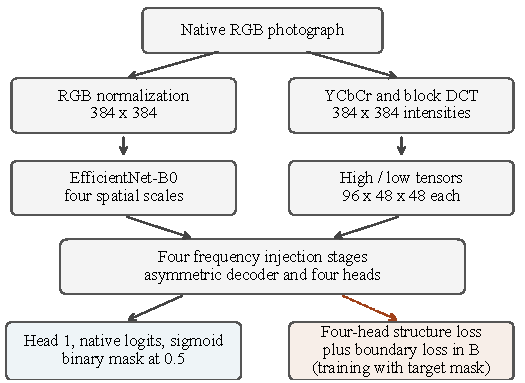
\includegraphics[width=\columnwidth]{figures/pipeline.pdf}
\caption{Shared FINet inputs and inference path. The boundary branch supplies an additional training loss to all four heads; it adds no inference module.}
\label{fig:pipeline}
\end{figure}

\subsection{Exact Baseline Structure Loss}
FINet's structure-loss code~\cite{finet} credits F3Net~\cite{f3net}. We retain FINet's implementation. For a batch of $B$ images with $N=384^2$ pixels each, define the weight map
\begin{equation}
 w_{nu}=1+5\left|
 \operatorname{AvgPool}_{31}(G)_{nu}-G_{nu}\right|.
 \label{eq:weights}
\end{equation}
Here $n$ indexes images and $u$ indexes pixels. The $31\times31$ average pool uses stride one and zero padding of 15 pixels. For head $h$, $P_h=\sigma(Z_h)$. The code's binary cross entropy (BCE) is a single scalar averaged over the entire batch:
\begin{equation}
 c_h=\frac{1}{BN}\sum_{n,u}
 \left[\operatorname{softplus}(Z_{hnu})-G_{nu}Z_{hnu}\right].
 \label{eq:basebce}
\end{equation}
This is the stable BCE-with-logits expression. Multiplying $c_h$ by $w$ and subsequently dividing by the sum of $w$ cancels the spatial weighting for BCE.

The intersection over union component remains weighted:
\begin{equation}
\begin{aligned}
 I_{hn}&=\sum_u w_{nu}P_{hnu}G_{nu},\\
 U_{hn}&=\sum_u w_{nu}
 \left(P_{hnu}+G_{nu}-P_{hnu}G_{nu}\right).
\end{aligned}
\label{eq:weighted_iou}
\end{equation}
The loss for one head is
\begin{equation}
 \ell_s(Z_h,G)=c_h+\frac{1}{B}\sum_n
 \left(1-\frac{I_{hn}+1}{U_{hn}+1}\right).
 \label{eq:structure}
\end{equation}
Both experiments use this implementation unchanged. A pixelwise weighted BCE would change the baseline and require a separate comparison.

\subsection{Differentiable Boundary Loss}
For a probability map $P$, define a local morphological gradient
\begin{equation}
 \mathcal B(P)_u=
 \max_{v\in\mathcal N_3(u)}P_v-
 \min_{v\in\mathcal N_3(u)}P_v,
 \label{eq:morph}
\end{equation}
where $\mathcal N_3(u)$ is the valid part of a $3\times3$ neighborhood. The minimum is computed by negating a maximum pool of the negated input. Pooling ignores positions outside the image, so constant maps have no artificial frame boundary.

For each image and head, set $Q=\mathcal B(\sigma(Z_h))$ and $T=\mathcal B(\mathbf1[G\geq0.5])$. Only $T$ is detached from the graph. The structure loss still receives the original soft mask. With $\widetilde Q=\operatorname{clip}(Q,\epsilon,1-\epsilon)$ and FP32 machine epsilon, the boundary BCE is
\begin{equation}
 \ell_{\mathrm{bce}}^{b}=
 -\frac1N\sum_u\!
 \left[T_u\log\widetilde Q_u+
 (1-T_u)\log(1-\widetilde Q_u)\right].
 \label{eq:boundarybce}
\end{equation}
Its companion Dice loss uses the unclamped $Q$:
\begin{equation}
 \ell_{\mathrm{dice}}^{b}
 =1-\frac{2\sum_u Q_uT_u+1}
 {\sum_u Q_u+\sum_u T_u+1}.
 \label{eq:boundarydice}
\end{equation}
The added loss $\ell_b$ is the batch average of
$\ell_{\mathrm{bce}}^{b}+\ell_{\mathrm{dice}}^{b}$. Maximum and minimum pooling are piecewise differentiable, so the probability maps still receive gradients. The complete objectives are
\begin{equation}
\begin{aligned}
 \mathcal L_A&=\sum_{h=1}^{4}\ell_s(Z_h,G),\\
 \mathcal L_B&=\mathcal L_A+
 \lambda\sum_{h=1}^{4}\ell_b(Z_h,G),\qquad \lambda=0.1.
\end{aligned}
\label{eq:objectives}
\end{equation}
At $\lambda=0$, the implementation skips boundary calculations and retains the baseline arithmetic. The experiment tests the stated coefficient and kernel; it does not establish that either is optimal.

\begin{table*}[!t]
\caption{Controlled model differences and differences between application domains}
\label{tab:comparison}
\centering\footnotesize
\begin{tabular}{L{0.19\textwidth}L{0.34\textwidth}L{0.34\textwidth}}
\hline
Within each domain & Baseline A & Boundary B\\
\hline
Training objective & Sum of four original structure losses & Same structure sum plus $0.1$ times four boundary losses\\
Full initial state & Identical encoder, random tensors and buffers & Same complete initial state as A\\
Inference network & Original FINet; 3,742,988 parameters & Same layers, tensor shapes and parameter count\\
Boundary computation & Skipped & $3\times3$ morphological BCE and Dice during training\\
Controlled settings & Fixed split, seed, sampling, augmentation and schedule & Same settings as A within the domain\\
Learned weights & Optimized with $\mathcal L_A$ & Separately optimized with $\mathcal L_B$\\
\hline
Between domains & Camouflaged objects & Industrial defects\\
\hline
Starting weights & ImageNet encoder plus random FINet components & Same initial FINet state, independently trained\\
Training data & COD10K and CAMO development split & Custom supervised MVTec split with labeled defects\\
Batch selection & Shuffled training images & Replacement sampling balanced by category and defect status\\
Augmentation & Original flip, crop, rotation, color and mask noise & Horizontal flip only; nearest neighbor mask resizing\\
Validation selection & Lowest native probability MAE & Highest macro Dice over categories' defective images\\
Final result availability & Both A and B complete; validation and one example & Baseline complete; final matched A/B unavailable\\
\hline
\end{tabular}
\end{table*}

\section{Experimental Protocol}
\subsection{Data Partitions and Separation}
The camouflage development set contains 4,040 image-mask pairs. Table~\ref{tab:camosplit} records the fixed source-stratified split. Original filenames, masks and content hashes are retained. Duplicate image pairs stay within one split. The two CAMO masks containing intermediate grayscale values are preserved for structure supervision.

\begin{table}[!t]
\caption{Camouflage development split}
\label{tab:camosplit}
\centering
\begin{tabular}{lrrr}
\hline
Source & Training & Validation & Total\\
\hline
COD10K & 2736 & 304 & 3040\\
CAMO & 900 & 100 & 1000\\
Combined & 3636 & 404 & 4040\\
\hline
\end{tabular}
\end{table}

The industrial experiment uses all 5,354 MVTec AD images from 15 categories. Table~\ref{tab:industrialsplit} separates normal and defective counts. Splitting is stratified by category, original split and defect type, with decoded duplicate images grouped together. Strata with fewer than three independent examples are held out entirely. Good images have empty masks; defective images use their native annotations.

\begin{table}[!t]
\caption{Custom supervised industrial split}
\label{tab:industrialsplit}
\centering
\begin{tabular}{lrrr}
\hline
Subset & Normal & Defective & Total\\
\hline
Training & 2866 & 862 & 3728\\
Validation & 615 & 198 & 813\\
Test & 615 & 198 & 813\\
\hline
\end{tabular}
\end{table}

Industrial models train independently from the common initial FINet state. Completed camouflage weights are never used for industrial fine-tuning or inference. The data handling changes with the domain, as summarized in Table~\ref{tab:comparison}. Because labeled defects enter industrial training, these results are not official normal-only MVTec anomaly benchmark scores.

\subsection{Optimization and Matched Budgets}
A and B share the optimization settings in Table~\ref{tab:settings}. Their common initialization includes every randomly initialized tensor and normalization buffer as well as the pretrained encoder. We use a single seed and deterministic cuDNN settings. Floating point behavior can still differ across software and hardware environments.

\begin{table}[!t]
\caption{Shared optimization settings}
\label{tab:settings}
\centering\footnotesize
\begin{tabular}{L{0.43\columnwidth}L{0.46\columnwidth}}
\hline
Setting & Value\\
\hline
Seed / input / batch & $123456$ / $384\times384$ / $4$\\
Training budget / precision & 200 epochs / FP32\\
Optimizer & Adam~\cite{adam}\\
Adam $\beta_1,\beta_2$ / $\epsilon$ & $(0.9,0.999)$ / $10^{-8}$\\
Initial / minimum learning rate & $2.6\times10^{-4}$ / $10^{-7}$\\
Weight decay & $4\times10^{-8}$\\
Loader workers / CPU threads & $2$ / $2$\\
cuDNN & Enabled, deterministic; benchmark disabled\\
Boundary coefficient / kernel & $0.1$ / $3\times3$ in B\\
Inference threshold & $0.5$ in both domains\\
Camouflage updates per epoch & $3636/4=909$\\
Industrial updates per epoch & $3728/4=932$\\
\hline
\end{tabular}
\end{table}

For zero-based epoch $e$ and $E=200$, the original cosine schedule is
\begin{equation}
 \eta_e=\eta_{\min}+
 \frac{\eta_{\max}-\eta_{\min}}{2}
 \left[1+\cos\left(\frac{\pi e}{E-1}\right)\right],
 \label{eq:schedule}
\end{equation}
with $e=0,\ldots,E-1$. The denominator is 199; the final training epoch uses $\eta_{\min}$. The scheduler advances after validation. Checkpoints retain model, Adam, scheduler and random generator states for recovery across GPU sessions.

Industrial training uses a joint stratum $s$ for each category and normal/defective status. If $n_s$ training images belong to stratum $s$, image $i$ has weight and selection probability
\begin{equation}
 w_i^{\mathrm{samp}}=\frac1{n_{s(i)}},
 \qquad q_i=\frac{w_i^{\mathrm{samp}}}{\sum_jw_j^{\mathrm{samp}}}.
 \label{eq:sampling}
\end{equation}
Each present stratum therefore has equal total selection probability. There are 3,728 replacement draws per epoch, with batch size four and the last incomplete batch dropped. A draw can repeat an image; an epoch does not guarantee that every industrial training image appears once.

The primary comparisons use the final weights from epoch 200. Checkpoints chosen by validation scores are kept separate because their selection epochs differ. Held out test images do not determine the boundary coefficient, threshold or checkpoint.

\section{Metrics and Auditable Outputs}
\label{sec:metrics}
\subsection{Native Restoration and Probability Storage}
For the first head, native probability and binary mask are
\begin{equation}
\begin{aligned}
 P^{\mathrm{native}}
 &=\sigma\!\left(\operatorname{Bilinear}_{H,W}(Z_1)\right),\\
 M_u&=\mathbf1[P^{\mathrm{native}}_u\geq0.5].
\end{aligned}
\label{eq:native}
\end{equation}
Final interpolation uses aligned corners. Logits are resized before sigmoid. The pipeline retains raw float32 probabilities without per-image minimum and maximum normalization, cleanup or forced foreground. Native masks and images must have matching dimensions before scores are computed.

\subsection{Region Metrics}
Let $Y$ be the native binary ground truth, and define
\begin{equation}
\begin{aligned}
 \mathrm{TP}&=|M\cap Y|,&
 \mathrm{FP}&=|M\setminus Y|,&
 \mathrm{FN}&=|Y\setminus M|.
\end{aligned}
\label{eq:counts}
\end{equation}
Dice and intersection over union (IoU) are
\begin{equation}
 D=\frac{2\mathrm{TP}}{2\mathrm{TP}+\mathrm{FP}+\mathrm{FN}},
 \qquad
 J=\frac{\mathrm{TP}}{\mathrm{TP}+\mathrm{FP}+\mathrm{FN}}.
 \label{eq:overlap}
\end{equation}
When both masks are empty, Dice and IoU are defined as one; when only one is empty, they are zero. The raw probability MAE of image $i$ and its mean over $K$ images are
\begin{equation}
\begin{aligned}
 a_i&=\frac1{H_iW_i}\sum_u|P^{\mathrm{native}}_{iu}-Y_{iu}|,\\
 \operatorname{MAE}&=\frac1K\sum_{i=1}^{K} a_i.
\end{aligned}
\label{eq:mae}
\end{equation}
Each image contributes equally to the mean, regardless of its pixel count. For camouflage validation only, $Y$ in \eqref{eq:mae} is the original grayscale mask divided by 255. The displayed test examples use binary targets. MAE has no special empty-mask override.

\subsection{Contour Metric and Boundary Definitions}
Evaluation uses a one-pixel inner contour
\begin{equation}
 \mathcal E(M)=M\setminus
 \operatorname{Erode}_{3\times3}(M).
 \label{eq:contour}
\end{equation}
Erosion uses eight neighbors and treats positions outside the image as zero. Let $d(x,S)$ be Euclidean distance to the nearest pixel in set $S$. With tolerance $\tau=2$ native pixels, contour precision, recall and F1 are
\begin{equation}
\begin{aligned}
 p_b&=\frac{|\{x\in\mathcal E(M):d(x,\mathcal E(Y))\leq\tau\}|}
 {|\mathcal E(M)|},\\
 r_b&=\frac{|\{y\in\mathcal E(Y):d(y,\mathcal E(M))\leq\tau\}|}
 {|\mathcal E(Y)|},\\
 F_b&=\frac{2p_br_b}{p_b+r_b}.
\end{aligned}
\label{eq:bf1}
\end{equation}
Both empty contours score one. A single empty contour, or nonempty contours with no matches, scores zero. This fixed tolerance is part of the project protocol and must accompany the scores.

\begin{table}[!t]
\caption{Three boundary operations with different purposes}
\label{tab:boundaries}
\centering\footnotesize
\begin{tabular}{L{0.27\columnwidth}L{0.62\columnwidth}}
\hline
Use & Definition and role\\
\hline
Training loss & $\mathcal B(P)$ on soft probabilities; differentiable local max minus min\\
Evaluation & $\mathcal E(M)$, an inner contour; Euclidean matching within two native pixels\\
Displayed edge & $\mathcal B(M)$ on a thresholded mask; a visualization, not the measured inner contour\\
\hline
\end{tabular}
\end{table}

The displayed edge is derived from the prediction; it is neither ground truth nor the inner contour measured by Boundary F1 (Table~\ref{tab:boundaries}). A broad predicted region can have high Dice even when few contour pixels fall within the strict tolerance.

\subsection{Output Contract}
Each prediction exports the seven artifacts in Table~\ref{tab:exports}; the application bundles them in a result ZIP. Scores use the float probability file, not a quantized preview. The registry separates industrial and camouflage checkpoint paths and rejects a missing or incompatible domain model. Industrial comparison requires a completed, matched pair. The camouflage comparison reported here uses both completed models.

\begin{table}[!t]
\caption{Per-prediction exports and their scientific meaning}
\label{tab:exports}
\centering\footnotesize
\begin{tabular}{L{0.35\columnwidth}L{0.54\columnwidth}}
\hline
Artifact & Meaning\\
\hline
\texttt{original.png} & Native RGB input\\
\texttt{probability.npy} & Native float32 $P$; source for measurements\\
\texttt{probability.png} & Truncated uint8 $255P$ for viewing\\
\texttt{binary.png} & $255\,\mathbf1[P\geq0.5]$\\
\texttt{overlay.png} & Foreground blend with opacity $0.45$ and RGB $(0,220,170)$\\
\texttt{boundary.png} & Morphological boundary of the binary prediction\\
\texttt{prediction.json} & Domain, checkpoint hash, epoch, threshold, dimensions and timing\\
\hline
\end{tabular}
\end{table}

\section{Results and Output Analysis}
\subsection{Verified Training Budgets}
The completed camouflage checkpoints and industrial baseline pass strict full-state loading (Table~\ref{tab:budgets}). The verified industrial boundary checkpoint is a partial recovery state. Later live updates have not been independently downloaded and verified, so they provide no final industrial checkpoint or A/B quality result.

\begin{table}[!t]
\caption{Verified saved training states}
\label{tab:budgets}
\centering\footnotesize
\begin{tabular}{llrr}
\hline
Domain & Variant & Epochs & Updates\\
\hline
Camouflage & A & 200 & 181800\\
Camouflage & B & 200 & 181800\\
Industrial & A & 200 & 186400\\
Industrial & B, recovery only & 6 & 5592\\
\hline
\end{tabular}
\end{table}

\subsection{Camouflage Validation}
At epoch 200, B has an absolute MAE decrease of 0.000409, or approximately 0.92 percent relative to A, while its common validation structure loss is slightly higher (Table~\ref{tab:validation}). Both validation loops evaluate the original structure objective, making that loss comparable. Total training losses differ in definition because B includes the boundary penalty. The table also records each run's minimum validation MAE and its selection epoch.

\begin{table}[!t]
\caption{Camouflage validation on the same 404 images}
\label{tab:validation}
\centering\footnotesize
\begin{tabular}{lrr}
\hline
Measurement & Baseline A & Boundary B\\
\hline
Final epoch & 200 & 200\\
Final MAE & 0.044454 & 0.044046\\
Final common structure loss & 2.590917 & 2.600930\\
Minimum validation MAE & 0.043109 & 0.042977\\
Epoch of minimum MAE & 153 & 182\\
\hline
\end{tabular}
\end{table}

The validation curves cross during training (Fig.~\ref{fig:validation}). Boundary MAE is higher at epochs 50 and 100 despite its lower final value. The lower final MAE is a single-seed validation observation, with no consistent advantage throughout training. These runs do not establish statistical significance, aggregate test improvement or overall contour improvement.

\begin{figure}[!t]
\centering
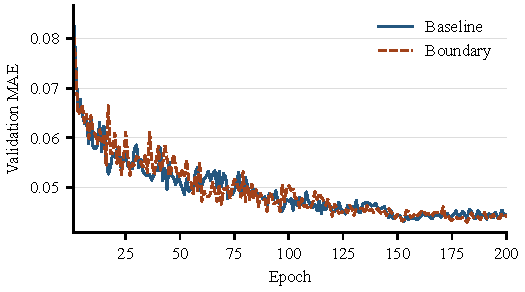
\includegraphics[width=\columnwidth]{figures/validation_mae.pdf}
\caption{Recorded native probability MAE over 200 camouflage training epochs. Both curves use the same 404-image validation split.}
\label{fig:validation}
\end{figure}

\subsection{Camouflaged Object Example}
The CAMO test photograph \texttt{camourflage\_00012}, of native size $632\times420$, is absent from the development manifest. Both epoch-200 models use threshold 0.5 on the same photograph and original binary annotation. The scores and counts in Table~\ref{tab:outputs} can be reproduced from the saved probabilities. We reuse this previously demonstrated image as an illustration; it was not randomly sampled.

Fig.~\ref{fig:camooutputs} shows the input and annotation alongside each binary mask, raw probability map and pixel error map. Green denotes true positives, red false positives and blue false negatives; background true negatives are dark. Probability images use the same fixed zero-to-one scale.

Both models recover most of the fish. B has 549 fewer false positive pixels and 273 fewer false negative pixels in this image. Dice rises from 0.9621 to 0.9671, while Boundary F1 rises from 0.3671 to 0.3958. Contour alignment remains weak relative to region overlap. One illustrative image cannot establish precise boundary recovery or a general advantage.

\begin{table*}[!t]
\caption{Native resolution scores and foreground error counts for the illustrated test examples}
\label{tab:outputs}
\centering\footnotesize
\begin{tabular}{llrrrrrrr}
\hline
Image & Model & Dice & IoU & MAE & Boundary F1 & TP & FP & FN\\
\hline
CAMO fish & A & 0.9621 & 0.9270 & 0.024941 & 0.3671 & 78814 & 5119 & 1084\\
CAMO fish & B & 0.9671 & 0.9363 & 0.021991 & 0.3958 & 79087 & 4570 & 811\\
\hline
Broken bottle & Industrial A & 0.8702 & 0.7702 & 0.011527 & 0.1884 & 31029 & 7156 & 2103\\
Bent metal nut & Industrial A & 0.9276 & 0.8650 & 0.002903 & 0.5000 & 8949 & 1214 & 183\\
Normal carpet & Industrial A & $1.0000^{a}$ & $1.0000^{a}$ & $<10^{-10}$ & $1.0000^{a}$ & 0 & 0 & 0\\
\hline
\multicolumn{9}{l}{\footnotesize $^{a}$Both masks are empty; the overlap and contour scores equal one by convention. These rows are individual examples.}\\
\end{tabular}
\end{table*}

\begin{figure*}[!t]
\centering
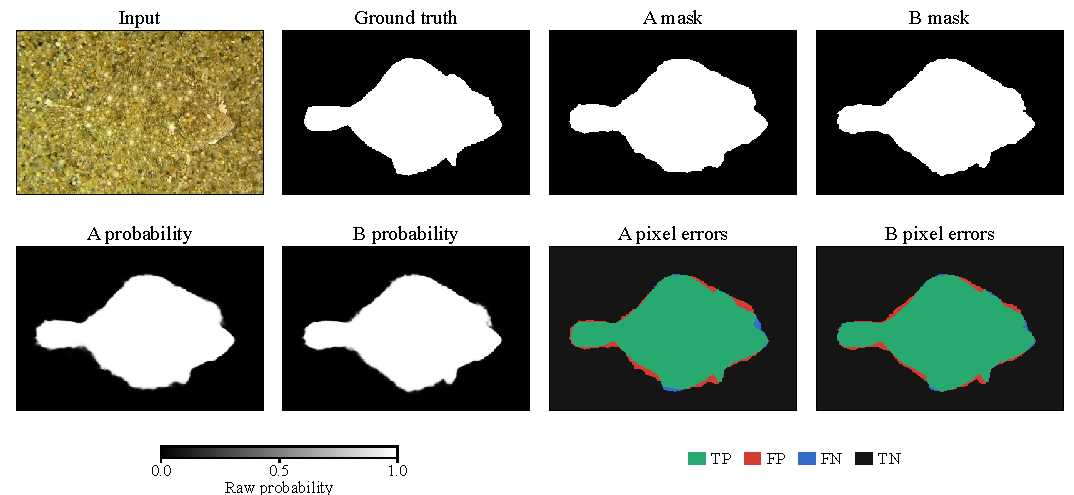
\includegraphics[width=\textwidth]{figures/camouflage_outputs.pdf}
\caption{Camouflage outputs from the two completed models. Top: input, ground truth, A mask and B mask. Bottom: A probability, B probability, A pixel errors and B pixel errors. The error maps distinguish TP, FP and FN at native resolution; no prediction normalization or cleanup is applied.}
\label{fig:camooutputs}
\end{figure*}

\subsection{Industrial Defect Examples}
Before inference, three test IDs were selected: the first registered broken bottle, bent metal nut and normal carpet. Their image and mask hashes were checked, and all IDs were excluded from training and validation. They have native sizes $900\times900$, $700\times700$ and $1024\times1024$, respectively. Only the independently trained industrial A checkpoint is used.

For the bottle, the target has 33,132 foreground pixels and the prediction has 38,185. The 7,156 false positives exceed the 2,103 false negatives, accounting for the foreground expansion in Fig.~\ref{fig:industrialoutputs}. Dice is 0.8702, but Boundary F1 is only 0.1884. The metal nut has 1,214 false positives and 183 false negatives, with Dice 0.9276 and Boundary F1 0.5000. Region scores alone miss the contour errors visible in both predictions.

The normal carpet has zero target and predicted foreground pixels. Its raw probability MAE is approximately $1.25648\times10^{-12}$, and its overlap and contour metrics equal one under the empty-mask convention. This correctly empty output and the two defective examples do not estimate accuracy across the 813-image test split or all 15 categories.

\begin{figure*}[!t]
\centering
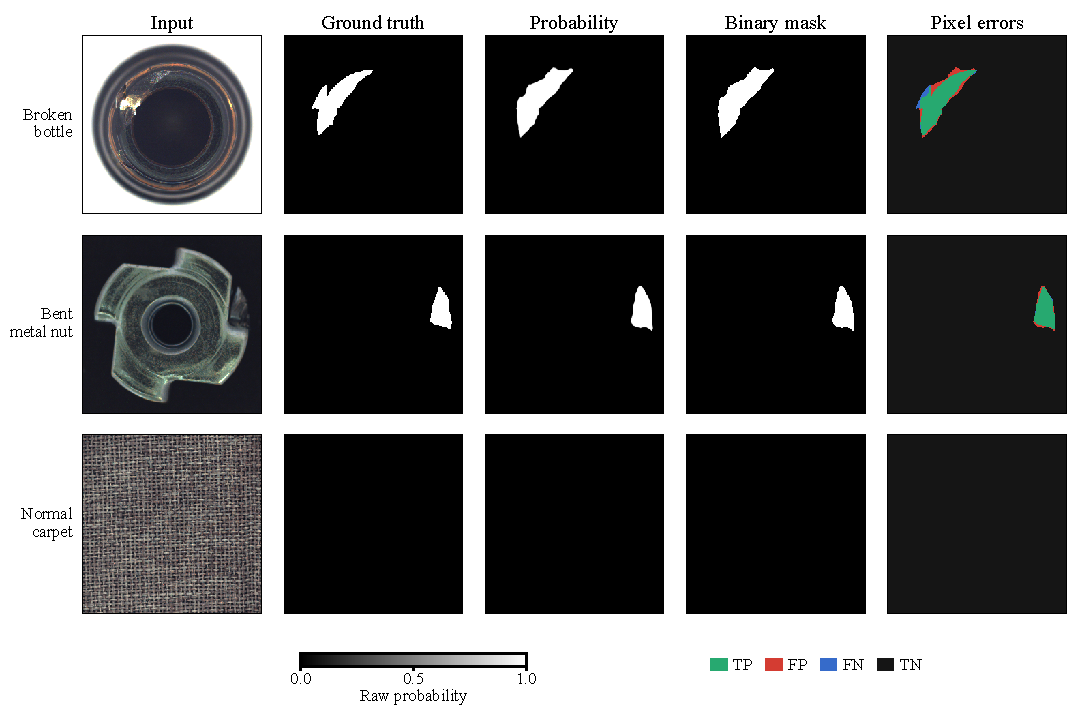
\includegraphics[width=\textwidth]{figures/industrial_outputs.pdf}
\caption{Industrial A outputs. Rows correspond to the broken bottle, bent metal nut and normal carpet. Columns contain the input, native ground truth, raw probability, binary mask and pixel errors. All probabilities share a fixed zero-to-one scale. Green, red and blue encode TP, FP and FN; the normal example has no foreground errors.}
\label{fig:industrialoutputs}
\end{figure*}

\section{Limitations and Remaining Evaluation}
Evaluation remains incomplete: aggregate camouflage test scores have not been independently verified, and the industrial boundary run has no verified final epoch-200 output. The validation measurements and individual examples cannot substitute for those results. Averaging the illustrations or using a partial checkpoint would not complete the evaluation.

The custom industrial split uses labeled defects during training and cannot be compared directly with official normal-only anomaly detection scores. Correctly empty predictions on normal images receive perfect overlap scores, so an eventual aggregate report must separate defective-only and all-image measurements by category. Otherwise many normal images could conceal poor defect localization.

Resizing to 384 pixels can remove small defects or displace native contours. A fixed tolerance of two native pixels is also relatively stricter on large photographs. The low contour scores in the examples identify a remaining weakness; they do not prove which preprocessing or modeling choice caused it. Higher-resolution or tiled inference would need a separate protocol.

We report one seed and one boundary coefficient/kernel. Consistent gains and optimal settings require repeated runs and validation-only ablations. Equal inference parameter counts do not establish equal speed or zero training overhead. Existing single-call CPU timings are insufficient for a latency benchmark.

The application displays candidate regions and preserves their provenance. It has no validated product acceptance rule. Production decisions would require a separate validation procedure and untouched evaluation data.

% Start the conclusion with enough space below the final output figure.
\newpage
\section{Conclusion}
Adding morphological boundary BCE and Dice loss to FINet's four training heads preserves the inference network. The comparison uses the exact baseline loss, preprocessing, sampler and native metric protocol specified here. Matched 200 epoch camouflage runs show a small final validation MAE decrease alongside a slightly higher common structure loss. In both domains, the native examples show substantial region overlap with weaker contour alignment. General improvement remains unresolved until full test evaluation and industrial boundary training are complete.

\begin{thebibliography}{00}
\bibitem{finet}
W. Liang, J. Wu, Y. Wu, X. Mu, and J. Xu, \lq\lq FINet: Frequency injection network for lightweight camouflaged object detection,\rq\rq\ \textit{IEEE Signal Process. Lett.}, vol. 31, pp. 526--530, 2024, doi: 10.1109/LSP.2024.3356416.
\bibitem{efficientnet}
M. Tan and Q. V. Le, \lq\lq EfficientNet: Rethinking model scaling for convolutional neural networks,\rq\rq\ in \textit{Proc. Int. Conf. Mach. Learn.}, vol. 97, 2019, pp. 6105--6114.
\bibitem{cod10k}
D.-P. Fan, G.-P. Ji, G. Sun, M.-M. Cheng, J. Shen, and L. Shao, \lq\lq Camouflaged object detection,\rq\rq\ in \textit{Proc. IEEE/CVF Conf. Comput. Vis. Pattern Recognit.}, 2020, pp. 2777--2787.
\bibitem{camo}
T.-N. Le, T. V. Nguyen, Z. Nie, M.-T. Tran, and A. Sugimoto, \lq\lq Anabranch network for camouflaged object segmentation,\rq\rq\ \textit{Comput. Vis. Image Underst.}, vol. 184, pp. 45--56, 2019, doi: 10.1016/j.cviu.2019.04.006.
\bibitem{mvtec}
P. Bergmann, M. Fauser, D. Sattlegger, and C. Steger, \lq\lq MVTec AD: A comprehensive real-world dataset for unsupervised anomaly detection,\rq\rq\ in \textit{Proc. IEEE/CVF Conf. Comput. Vis. Pattern Recognit.}, 2019, pp. 9584--9592, doi: 10.1109/CVPR.2019.00982.
\bibitem{dct}
N. Ahmed, T. Natarajan, and K. R. Rao, \lq\lq Discrete cosine transform,\rq\rq\ \textit{IEEE Trans. Comput.}, vol. C-23, no. 1, pp. 90--93, 1974, doi: 10.1109/T-C.1974.223784.
\bibitem{f3net}
J. Wei, S. Wang, and Q. Huang, \lq\lq F$^3$Net: Fusion, feedback and focus for salient object detection,\rq\rq\ in \textit{Proc. AAAI Conf. Artif. Intell.}, vol. 34, no. 07, 2020, pp. 12321--12328, doi: 10.1609/aaai.v34i07.6916.
\bibitem{adam}
D. P. Kingma and J. Ba, \lq\lq Adam: A method for stochastic optimization,\rq\rq\ in \textit{Proc. Int. Conf. Learn. Represent.}, 2015.
\end{thebibliography}
\end{document}
